\section{相对论重离子对撞机——RHIC}

相对论重离子对撞机位于美国纽约长岛上的布鲁克海文国家实验室(Brookhaven National Laboratory, BNL)内,
可以进行质心系能量最高为 \sNNerbai 的重离子对撞和质心系能量最高为 $\sqrt{s_{\mathrm{NN}}} = $ 510 GeV的极化质子-质子对撞。

RHIC是世界上第一台可以进行重离子对撞的对撞机,也是现存的唯一一台可以进行极化质子-质子对撞的对撞机。在RHIC上可以进行多种离子的对撞,以金-金对撞为例,其质心系能量最高可以达到 \sNNerbai 。对重离子对撞来说,因为RHIC具有可对撞离子种类多和能量范围宽的特点,可以进行多种离子系统和束流能量扫描,对研究夸克胶子等离子体的性质有着很大的帮助。

RHIC主要由两条独立的长约3.8公里(2.4英里)的加速储存环构成,离子或者质子可以在其中被加速到接近光速,并且在两个环的交叉点发生头对头碰撞。在整个RHIC环上两个环一共有6个交叉点可以来进行束流的头对头碰撞,束流在两条环里的运行方向相反,RHIC上的各个实验就位于这些交叉点的位置。离子或者质子在两个环当中以束流(Beam)的形式存在。其中沿着顺时针方向运行的束流被称作Blue Beam,沿逆时针方向运行的束流被称作Yellow Beam。从RHIC建成至今,一共有过STAR,PHENIX,PHOBOS 和 BRAHMS四个实验,分别位于RHIC环的 6点,8点,10点,和 2点钟方向。截止到本文写作时间(2022年)RHIC上仅有STAR实验还在运行取数,而RHIC也即将在不久的将来停机升级成电子-离子对撞机(e-RHIC)。

RHIC综合装置的示意图如图 \ref{fig:RHIC} 所示。接下来将以金离子为例介绍RHIC的离子加速过程。金原子在经历整个过程后外层电子被剥离并被加速到所需要的束流能量。整个离子加速过程由三部分组成,
\begin{figure}[htb]
    \begin{center}
    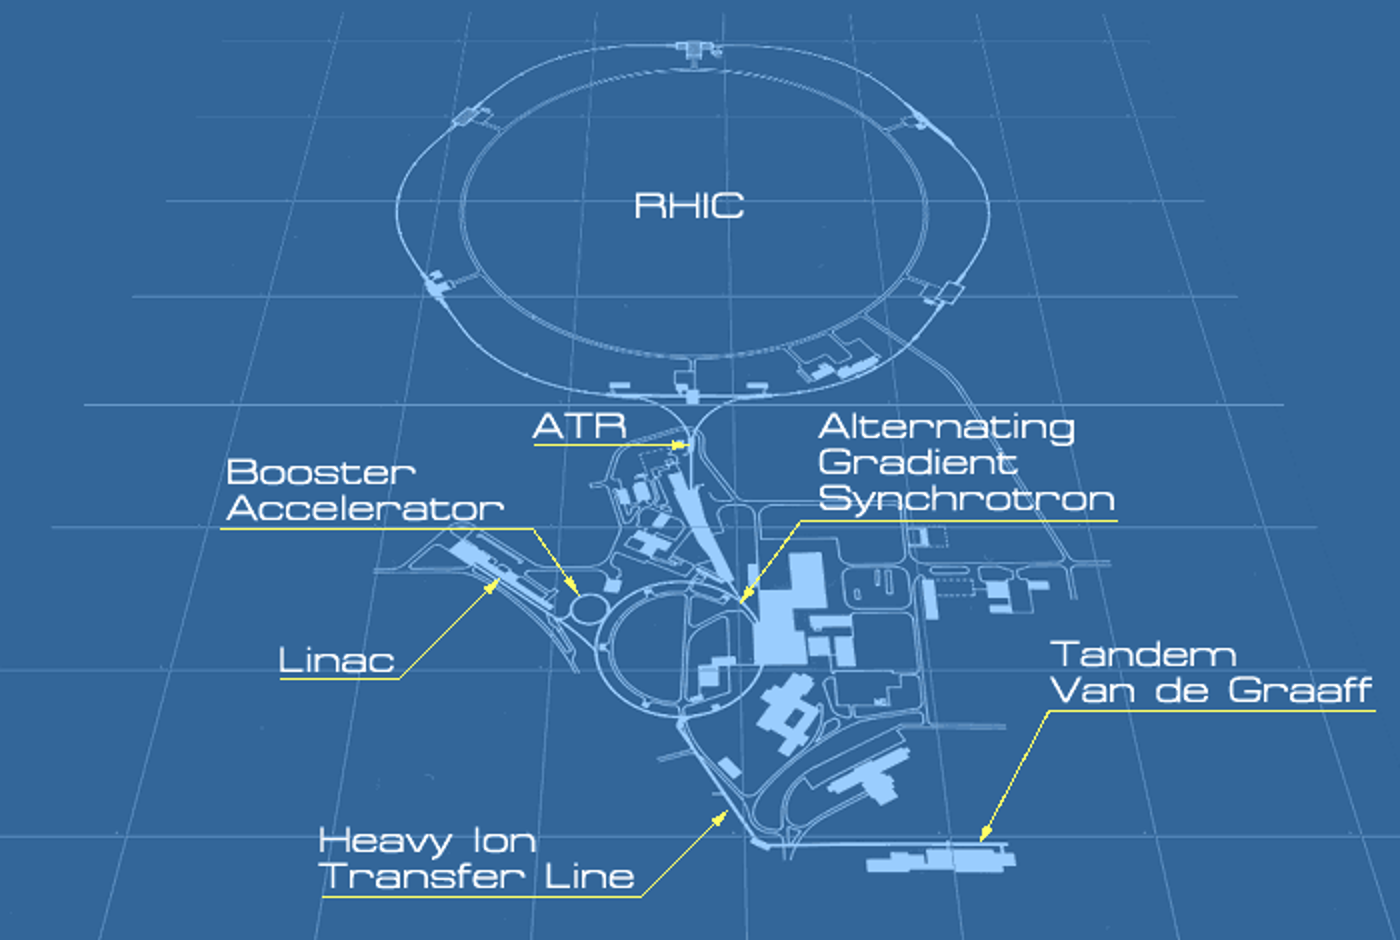
\includegraphics[width=0.8\textwidth,clip]{figures/Chapter2/RHIC.png}
    \end{center}
    \caption[相对论重离子对撞机(RHIC)综合装置示意图]{相对论重离子对撞机(RHIC)综合装置示意图}
    \label{fig:RHIC}
\end{figure}

金离子首先由脉冲溅射离子源(Pulser Sputter Ion Source)产生,带负电荷的金离子在串列范德格拉夫加速器(Tandem Van de Graaff)中被剥离一部分电子,变成电荷量为+32的金离子并被加速到 1 MeV/$\mu$。之后电荷量为+32的金离子经过传输线被输送到增强器(Booster Synchrotron)中,在增强器中金离子被加速到 95 MeV/$\mu$ 并且外层电子被进一步剥离变成电荷量为+77的金离子并被注入到交变梯度同步加速器(Alternating Gradient Synchrotron, AGS)当中进行进一步的加速。电荷量为+77的金离子在交变梯度同步加速器被加速达到RHIC的注入能量 10.8 MeV/$\mu$后被送入AGS至RHIC的束流转移线(AGS-to-RHIC Beam Transfer Line)。金离子在束流转移线当中被剥离掉最后的电子成为电荷量为+79的离子后注入到RHIC当中,最后在RHIC中加速到对撞所需要的束流能量。